\documentclass{article}
\usepackage{amsmath}
\usepackage{titlesec}
\usepackage[mathletters]{ucs}
\usepackage[utf8x]{inputenc}
\usepackage[margin=1.5in]{geometry}
\usepackage{enumerate}
\newtheorem{theorem}{Theorem}
\usepackage[dvipsnames]{xcolor}
\usepackage{pgfplots}
\pgfplotsset{compat=1.18}
\setlength{\parindent}{0cm}
\usepackage{graphics}
\usepackage{graphicx} % Required for including images
\usepackage{subcaption}
\usepackage{bigintcalc}
\usepackage{pythonhighlight} %for pythonkode \begin{python}   \end{python}
\usepackage{appendix}
\usepackage{arydshln}
\usepackage{physics}
\usepackage{booktabs} 
\usepackage{adjustbox}
\usepackage{mdframed}
\usepackage{relsize}
\usepackage{physics}
\usepackage[thinc]{esdiff}
\usepackage{esint}  %for lukket-linje-integral
\usepackage{xfrac} %for sfrac
\usepackage{hyperref} %for linker, må ha med hypersetup
\usepackage[noabbrev, nameinlink]{cleveref} % to be loaded after hyperref
\usepackage{amssymb} %\mathbb{R} for reelle tall, \mathcal{B} for "matte"-font
\usepackage{listings} %for kode/lstlisting
\usepackage{verbatim}
\usepackage{graphicx,wrapfig,lipsum,caption} %for wrapping av bilder
\usepackage{mathtools} %for \abs{x}
\usepackage[english]{babel}
\usepackage{cancel}
\definecolor{codegreen}{rgb}{0,0.6,0}
\definecolor{codegray}{rgb}{0.5,0.5,0.5}
\definecolor{codepurple}{rgb}{0.58,0,0.82}
\definecolor{backcolour}{rgb}{0.95,0.95,0.92}
\lstdefinestyle{mystyle}{
    backgroundcolor=\color{backcolour},   
    commentstyle=\color{codegreen},
    keywordstyle=\color{magenta},
    numberstyle=\tiny\color{codegray},
    stringstyle=\color{codepurple},
    basicstyle=\ttfamily\footnotesize,
    breakatwhitespace=false,         
    breaklines=true,                 
    captionpos=b,                    
    keepspaces=true,                 
    numbers=left,                    
    numbersep=5pt,                  
    showspaces=false,                
    showstringspaces=false,
    showtabs=false,                  
    tabsize=2
}

\lstset{style=mystyle}
\author{Oskar Idland}
\title{Oblig 1}
\date{}
\begin{document}
\maketitle
%\tableofcontents
\newpage

\subsection*{Problem 1}
\subsection*{a)}
\begin{figure}[h!]
\centering
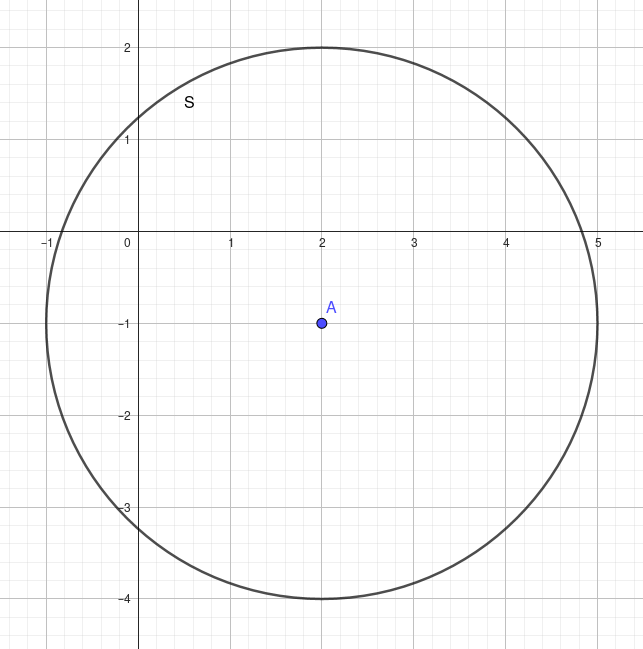
\includegraphics[width = .5\textwidth]{1a.png}
\caption{Curve: $\left\{z ∈ ℂ : \left|z\right| = 1\right\}$. Function: $f(z) = 3(z+2-i)$}
\label{fig: 1a}
\end{figure}

\subsection*{b)}
\begin{figure}[h!]
\centering
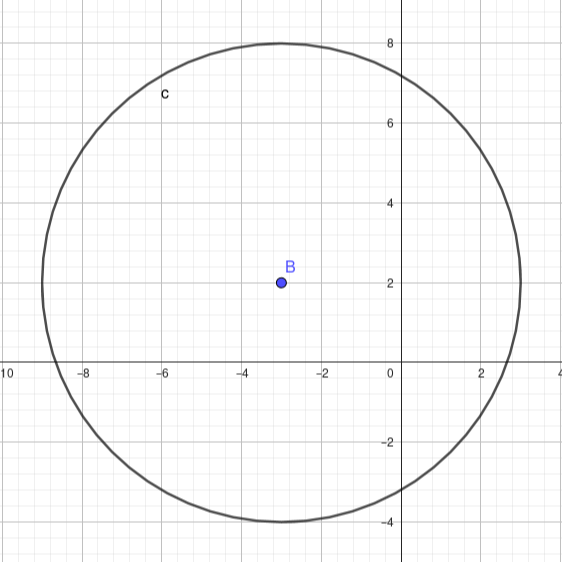
\includegraphics[width = \textwidth]{1b.png}
\caption{$z-3+2i$ represents a circle with center at $(-3,2)$. $\left|z\right|$ can have values from 1 to 3}
\label{fig: }
\end{figure}

\subsection*{c)}

\subsection*{d)}




\subsection*{Problem 2}
\subsection*{a)}
We begin with the convergence test. 
\[
\lim_{n \to ∞}\left|\frac{a_{n+1}}{a_n}\right| < 1
\]
\[
\lim_{n \to ∞} \left|\frac{3^{n}(z+4-2i)^{2n + 2}}{3^{n+1}(z+4-2i)^{2n}}\right| = \lim_{n \to ∞} \left|\frac{(z+4-2i)^2}{3}\right| < 1
\]
\[
\lim_{n \to ∞} \left|z + 4 - 2i\right| < \sqrt{3}
\]

\subsection*{b)}
\[
\lim_{n \to ∞} \left|\frac{\left(z-3+i\right)(n^2 + 2n)}{(n+1)^2 + 4n^2}\right| = \lim_{n \to ∞} \left|\frac{(z-3+i)(n^2 + 2n)}{n^2 + 2n + 1 + 4n^2}\right|
\]

\subsection*{c)}
\[
\lim_{n \to ∞} \left|\frac{\ln (n+1)nz^{n+1}}{\ln (n)z^{n}(n+1)}\right| = \lim_{n \to ∞} \left|\frac{\ln (n+1)n z}{\ln (n)(n+1)}\right| < 1
\]




\subsection*{Problem 3}
\subsection*{a)}

\subsection*{b)}

\subsection*{c)}

\end{document}